%       --- Design and Rationale --- Design and Rationale --- Design and Rationale --- Design and Rationale --- Design and Rationale --- Design and Rationale
\chapter{Design and Rationale - example middle chapter} % --- Design and Rationale --- Design and Rationale --- Design and Rationale --- Design and Rationale
%       --- Design and Rationale --- Design and Rationale --- Design and Rationale --- Design and Rationale --- Design and Rationale --- Design and Rationale

%       --- Design --- Design --- Design --- Design --- Design --- Design --- Design --- Design --- Design --- Design --- Design --- Design --- Design ---
\section{Design} % --- Design --- Design --- Design --- Design --- Design --- Design --- Design --- Design --- Design --- Design --- Design --- Design ---
%       --- Design --- Design --- Design --- Design --- Design --- Design --- Design --- Design --- Design --- Design --- Design --- Design --- Design ---

\begin{tcolorbox}[      % Delete me later
    boxrule=0pt,        % Delete me later
    colback=white,      % Delete me later
    coltext=red         % Delete me later
]                       % Delete me later
    Describe the design of the system at a high level. The system should support the use cases described in the previous chapter.
    
    ---C4 system context and container diagrams go in this section. See: https://c4model.com/ (C4 Model Website)

    \vspace{15pt}       % Delete me later
    \begin{center}      % Delete me later
    \textbf{Don't forget to delete this explanatory red text/block introduction, and replace it with your text in black.}
    \end{center}        % Delete me later
\end{tcolorbox}         % Delete me later

\pagebreak

%       --- Use Case Overview --- Use Case Overview --- Use Case Overview --- Use Case Overview --- Use Case Overview --- Use Case Overview ---
\section{Use Case Overview} % --- Use Case Overview --- Use Case Overview --- Use Case Overview --- Use Case Overview --- Use Case Overview ---
%       --- Use Case Overview --- Use Case Overview --- Use Case Overview --- Use Case Overview --- Use Case Overview --- Use Case Overview ---

\begin{tcolorbox}[      % Delete me later
    boxrule=0pt,        % Delete me later
    colback=white,      % Delete me later
    coltext=red         % Delete me later
]                       % Delete me later
    Brief explanation of how use cases were derived from user stories.

    \vspace{15pt}       % Delete me later
    \begin{center}      % Delete me later
    \textbf{Don't forget to delete this explanatory red text/block introduction, and replace it with your text in black.}
    \end{center}        % Delete me later
\end{tcolorbox}         % Delete me later

%       --- Use Case Descriptions --- Use Case Descriptions --- Use Case Descriptions --- Use Case Descriptions ---
\section{Use Case Descriptions} % --- Use Case Descriptions --- Use Case Descriptions --- Use Case Descriptions ---
%       --- Use Case Descriptions --- Use Case Descriptions --- Use Case Descriptions --- Use Case Descriptions ---

\begin{figure}[h!]
    \centering
    \begin{tcolorbox}[title=Use Case 1: EXAMPLE Explore Campus Virtually]
        \textbf{Actor:} Prospective Student
        \textbf{Preconditions:} User is on the landing page.

        \textbf{Main Flow:}
        \begin{enumerate}
            \item User selects “Start Virtual Tour”.
            \item System displays a map of campus buildings.
            \item User clicks on a building icon.
            \item System opens a 3D or 360° tour of that building.
        \end{enumerate}

        \textbf{Alternate Flow:} If media fails to load, fallback images are shown.
        \textbf{Postconditions:} User has explored one or more buildings virtually.
    \end{tcolorbox}

    \vspace*{-5pt}
    \caption{Use Case 1: EXAMPLE Explore Campus Virtually}
    \label{fig:usecase1}
\end{figure}

\vspace{1em}

\begin{figure}[h!]
    \centering
    \begin{tcolorbox}[title=Use Case 2: EXAMPLE View Campus Safety Information]
        \textbf{Actor:} Parent of Prospective Student
        \textbf{Preconditions:} User is on the main information page.

        \textbf{Main Flow:}
        \begin{enumerate}
            \item User navigates to the “Safety Info” section.
            \item System displays emergency contacts and safety resources.
        \end{enumerate}

        \textbf{Postconditions:} User is informed about campus safety services.
    \end{tcolorbox}

    \vspace*{-5pt}
    \caption{Use Case 2:  EXAMPLE View Campus Safety Information}
    \label{fig:usecase2}
\end{figure}

\pagebreak

%         --- Use Case Diagram --- Use Case Diagram --- Use Case Diagram --- Use Case Diagram --- Use Case Diagram ---
%         --- Use Case Diagram --- Use Case Diagram --- Use Case Diagram --- Use Case Diagram --- Use Case Diagram ---
\section{Use Case Diagram(s)} % --- Use Case Diagram --- Use Case Diagram --- Use Case Diagram --- Use Case Diagram ---

\begin{tcolorbox}[      % Delete me later
    boxrule=0pt,        % Delete me later
    colback=white,      % Delete me later
    coltext=red         % Delete me later
]                       % Delete me later
    Include at least one UML use case diagram that includes an overview and relationship of your text use cases.
    \vspace{\baselineskip}
    (You can use the tikz-uml package to draw a Unified Modeling Language models or you use an UML editor of your choice and upload the pictures here.)
    
    \vspace{15pt}       % Delete me later
    \begin{center}      % Delete me later
    \textbf{Don't forget to delete this explanatory red text/block introduction, and replace it with your text in black.}
    \end{center}        % Delete me later
\end{tcolorbox}         % Delete me later



\begin{figure}[h!] % Use Case Diagram ---
    \centering
    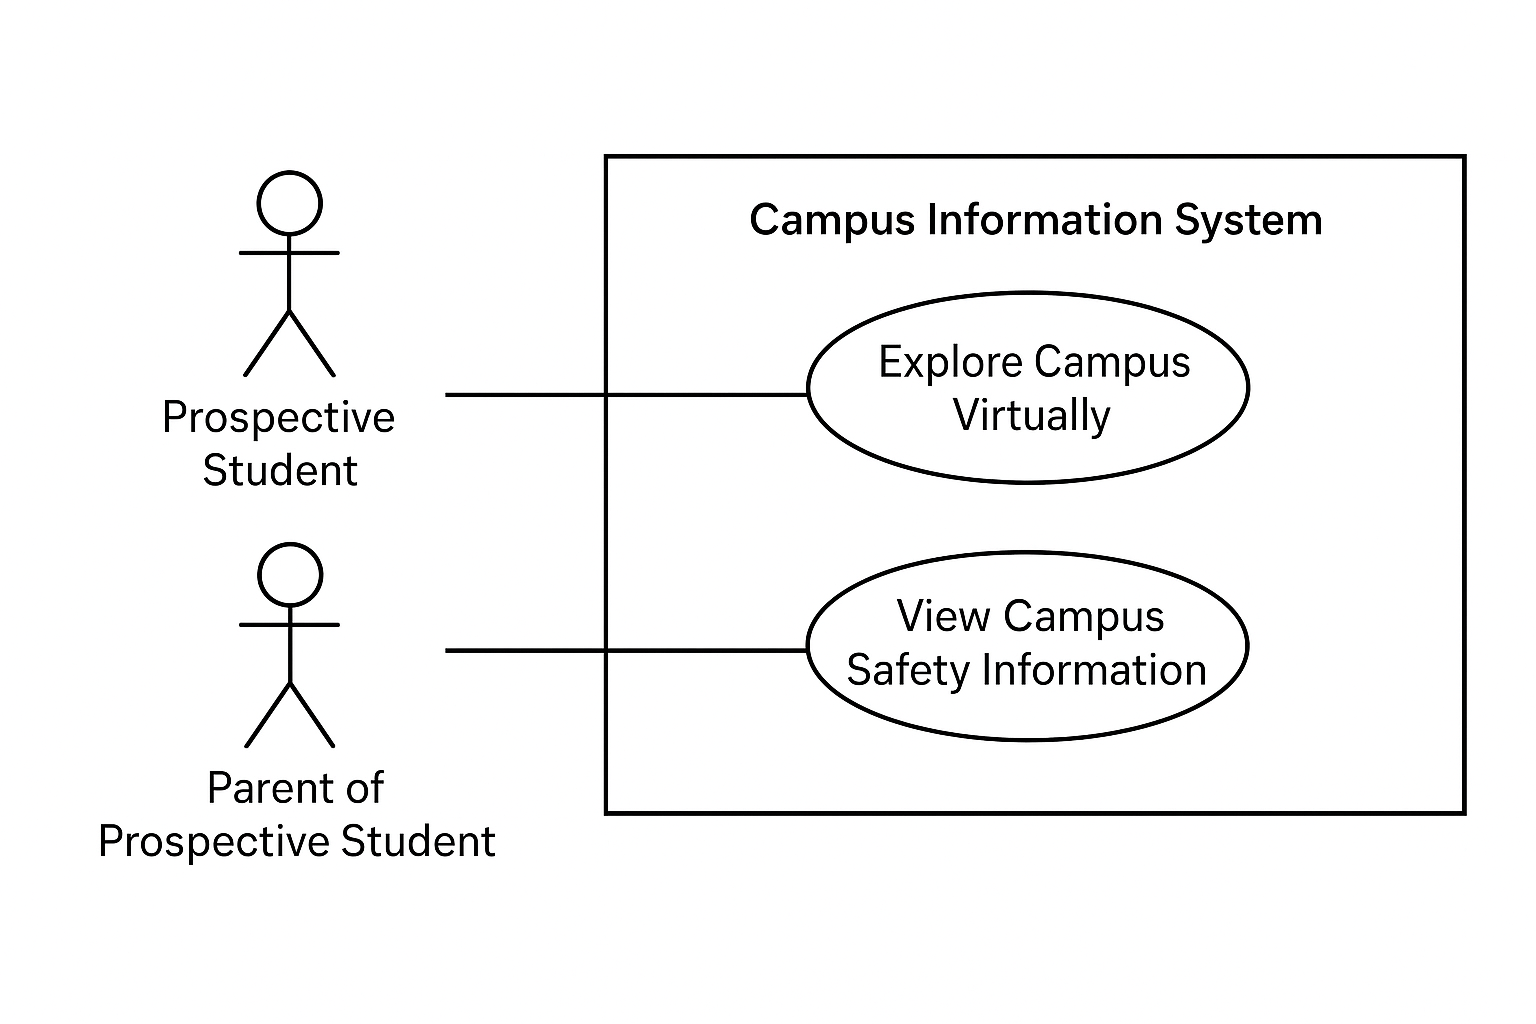
\includegraphics[width=0.8\linewidth]{pictures/example-use-case-diagram.png}

% For some reasons drawing UML Use Case diagrams with tik looks ugly, so picture included (above)
%    \begin{tikzpicture}
%        \begin{umlpackage}{Campus Information System}
%            % Use cases inside
%            \umlusecase[x=4,y=3.5,width=4cm]{Explore Campus Virtually}
%            \umlusecase[x=4,y=1,width=4cm]{View Campus Safety Information}
%        \end{umlpackage}
%        
%        % Actors outside (aligned left)
%        \umlactor[x=0,y=3.5]{Prospective Student}
%        \umlactor[x=0,y=1]{Parent of Prospective Student}
%        
%        % Associations (straight connections)
%        \umlassoc{Prospective Student}{usecase-1}
%        \umlassoc{Parent of Prospective Student}{usecase-2}
%    \end{tikzpicture}

    \caption{EXAMPLE UML Use Case Diagram: Campus Information System}
    \label{fig:uml_use_case_diagram}
\end{figure}


    
\pagebreak

%       --- Class Diagram --- Class Diagram --- Class Diagram --- Class Diagram --- Class Diagram ---
\section{Class Diagram} % --- Class Diagram --- Class Diagram --- Class Diagram --- Class Diagram ---
%       --- Class Diagram --- Class Diagram --- Class Diagram --- Class Diagram --- Class Diagram ---

\begin{tcolorbox}[      % Delete me later
    boxrule=0pt,        % Delete me later
    colback=white,      % Delete me later
    coltext=red         % Delete me later
]                       % Delete me later
    Include at least one UML Class Diagram that includes an overview over your system.
    
    \vspace{\baselineskip}
    (You can use the tikz-uml package to draw a Unified Modeling Language models or you use an UML editor of your choice and upload the pictures here.)

    \vspace{15pt}       % Delete me later
    \begin{center}      % Delete me later
    \textbf{Don't forget to delete this explanatory red text/block introduction, and replace it with your text in black.}
    \end{center}        % Delete me later
\end{tcolorbox}         % Delete me later


\begin{figure}[h!] % Class Diagram ---
    \centering
    \begin{center}
        \begin{tikzpicture}
            \begin{umlpackage}{System}
                \begin{umlpackage}{UserRegistration}
                    \umlclass[template=T]{User}{
                        age : uint
                        \\
                        birthday : Date
                    }{}
                    \umlclass[y=-3]{Department}{
                        d : double
                    }{
                        \umlvirt{
                            setB(b : B) : void
                        } 
                        \\ 
                        getB() : B
                    }
                \end{umlpackage}
            
                \begin{umlpackage}[x=10,y=-6]{Facility}
                    \umlinterface{BaseBuilding}{
                        n : uint 
                        \\ 
                        s : string
                    }{}
                \end{umlpackage}
            
                \umlclass[x=2,y=-10]{DataType}{
                    n : uint
                }{}
            \end{umlpackage}
            
            \umlassoc[geometry=-|-, arg1=tata, mult1=*, pos1=0.3, arg2=toto, mult2=1, pos2=2.9, align2=left]{BaseBuilding}{Department}
            \umlunicompo[geometry=-|, arg=titi, mult=*, pos=1.7, stereo=vector]{DataType}{BaseBuilding}
            \umlimport[geometry=|-, anchors=90 and 50, name=import]{Facility}{UserRegistration}
            \umlaggreg[arg=tutu, mult=1, pos=0.8, angle1=30, angle2=60, loopsize=2cm]{DataType}{DataType}
            \umlinherit[geometry=-|]{DataType}{Department}
            \umlnote[x=2.5,y=-6, width=3cm]{Department}{Every department has at least one user}
            \umlnote[x=7.5,y=-2]{import-2}{This note is about the import relationship.}
        \end{tikzpicture}
    \end{center}
    \caption{EXAMPLE Class Diagram: System}
    \label{fig:class_diagram}
\end{figure}

\pagebreak

%       --- Sequence Diagram --- Sequence Diagram --- Sequence Diagram --- Sequence Diagram --- Sequence Diagram ---
\section{Sequence Diagram} % --- Sequence Diagram --- Sequence Diagram --- Sequence Diagram --- Sequence Diagram ---
%       --- Sequence Diagram --- Sequence Diagram --- Sequence Diagram --- Sequence Diagram --- Sequence Diagram ---

\begin{figure}[h!] % Sequence Diagram ---
    \centering
    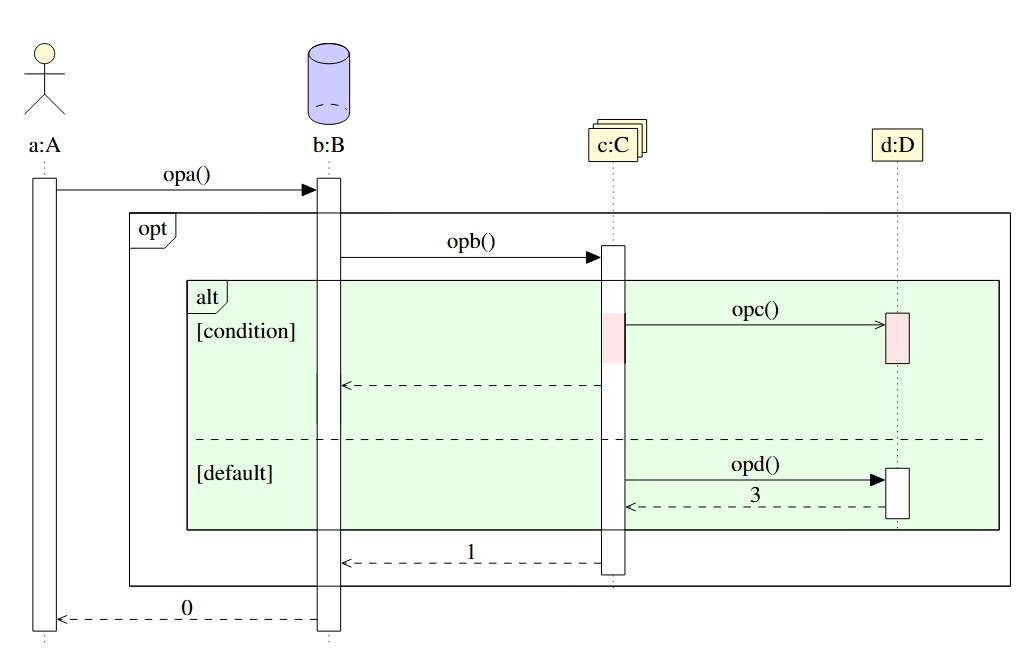
\includegraphics[width=0.8\linewidth]{pictures/example-sequence-diagram.jpg}
    
%    For some reason, this TIK creates two if-then-else errors 
%    \begin{tikzpicture}
%        \begin{umlseqdiag}
%            \umlactor[class=A]{a}
%            \umldatabase[class=B, fill=blue!20]{b}
%            \umlmulti[class=C]{c}
%            \umlobject[class=D]{d}
%            \begin{umlcall}[op=opa(), type=synchron, return=0]{a}{b}
%                \begin{umlfragment}
%                    \begin{umlcall}[op=opb(), type=synchron, return=1]{b}{c}
%                        \begin{umlfragment}[type=alt, label=condition, inner xsep=8, fill=green!10]
%                            \begin{umlcall}[op=opc(), type=asynchron, fill=red!10]{c}{d}
%                            \end{umlcall}
%                            \begin{umlcall}[type=return]{c}{b}
%                            \end{umlcall}
%                            \umlfpart[default]
%                            \begin{umlcall}[op=opd(), type=synchron, return=3]{c}{d}
%                            \end{umlcall}
%                        \end{umlfragment}
%                    \end{umlcall}
%                \end{umlfragment}
%            \end{umlcall}
%        \end{umlseqdiag}
%    \end{tikzpicture}
    \caption{EXAMPLE Sequence Diagram: Security Hand Shake}
    \label{fig:sequence_diagram}
\end{figure}

\pagebreak

%       --- State Diagram --- State Diagram --- State Diagram --- State Diagram --- State Diagram --- State Diagram ---
\section{State Diagram} % --- State Diagram --- State Diagram --- State Diagram --- State Diagram --- State Diagram ---
%       --- State Diagram --- State Diagram --- State Diagram --- State Diagram --- State Diagram --- State Diagram ---

\begin{figure}[h!] % State Diagram ---
    \centering
    \begin{center}
        \begin{tikzpicture}
            \begin{umlstate}[name=Amain]{Initialization Process}
                \begin{umlstate}[name=Bgraph, fill=red!20]{graphe B}
                    \umlstateinitial[name=Binit]
                    \umlbasicstate[y=-4, name=test1, fill=white]{test1}
                    \umltrans{Binit}{test1}
                    \umltrans[recursive=20|60|2.5cm, recursive direction=right to top, arg={op1}, pos=1.5]{test1}{test1}
                    \umltrans[recursive=160|120|2.5cm, recursive direction=left to top, arg={op2}, pos=1.5]{test1}{test1}
                    \umltrans[recursive=-160|-120|2.5cm, recursive direction=left to bottom, arg={op3}, pos=1.5]{test1}{test1}
                    \umltrans[recursive=-20|-60|2.5cm, recursive direction=right to bottom, arg={op4}, pos=1.5]{test1}{test1}
                    \umlbasicstate[y=-8, name=test2, fill=white]{test2}
                    \umltrans[recursive=-160|-120|2.5cm, recursive direction=left to bottom, arg={op5}, pos=1.5]{test2}{test2}
                    \umltrans{test1}{test2}
                    \umlstatefinal[x=3, y=-7.75, name=Bfinal]
                    \umltrans{test2}{Bfinal}
            \end{umlstate}
                \umlstateinitial[x=6, y=1, name=Ainit]
                \umlVHtrans[anchor2=40]{Ainit}{Bgraph}
                \umlstatefinal[x=6, y=-3.5, name=Afinal]
                \umlHVtrans[anchor1=30]{Bgraph}{Afinal}
                \umlbasicstate[x=6, y=-6, name=visu, fill=green!20]{Visualisation}
                \umlHVtrans{Bfinal}{visu}
                \umltrans{visu}{Afinal}
                \umltrans[recursive=-20|-60|2.5cm, recursive direction=right to bottom, arg=a, pos=1.5]{visu}{visu}
            \end{umlstate}
        \end{tikzpicture}
    \end{center}
    \caption{EXAMPLE State Diagram: Initialization Process}
    \label{fig:state_diagram}
\end{figure}

\pagebreak

%       --- Component Diagram --- Component Diagram --- Component Diagram --- Component Diagram --- Component Diagram --- Component Diagram ---
\section{Component Diagram} % --- Component Diagram --- Component Diagram --- Component Diagram --- Component Diagram --- Component Diagram ---
%       --- Component Diagram --- Component Diagram --- Component Diagram --- Component Diagram --- Component Diagram --- Component Diagram ---

\begin{figure}[h!] % Component Diagram ---
    \centering
    \begin{center}
        \begin{tikzpicture}
            \begin{umlcomponent}{A}
                \umlbasiccomponent{B}
                \umlbasiccomponent[y=-2]{C}
                \umlrequiredinterface[interface=C-interface]{C}
                \umlprovidedinterface[interface=B-interface, with port, distance=3cm, padding=2.5cm]{B}
            \end{umlcomponent}
            \umlbasiccomponent[x=-10,y=1]{D}
            \umlbasiccomponent[x=3,y=-7.5]{E}
            \umlbasiccomponent[x=-2, y=-9]{F}
            \umlbasiccomponent[x=-7,y=-8]{G}
            \umlbasiccomponent[x=-7,y=-11]{H}    
            \umlassemblyconnector[interface=DA, with port, name=toto]{D}{A}
            \umldelegateconnector{A-west-port}{B-west-interface}
            \umlVHVassemblyconnector[interface=AE, with port]{A}{E}
            \umlHVHassemblyconnector[interface=EF, with port, first arm]{E}{F}
            \umlHVHassemblyconnector[interface=GHF, with port, arm2=-2cm, last arm]{G}{F}
            \umlHVHassemblyconnector[with port, arm2=-2cm, last arm]{H}{F}
            
            \umlnote[x=-4, y=4, width=3.4cm]{B-west-interface}{I am the node named B-west-interface}
            \umlnote[x=2, y=4, width=3.4cm]{C-east-interface}{I am the node named C-east-interface}
            \umlnote[x=-8.5, y=-2, width=3.4cm]{toto-interface}{I am the node named toto-interface}
            \umlnote[x=-5.5, y=-4.5, width=3.4cm]{A-south-port}{I am the node named A-south-port}
            \umlnote[x=-1, y=-6, width=3.4cm]{AE-interface}{I am the node named AE-interface}
            \umlnote[x=2, y=-11, width=3.4cm]{F-east-port}{I am the node named F-east-port}
        \end{tikzpicture}
    \end{center}
    \caption{EXAMPLE Component Diagram: Major Components}
    \label{fig:component_diagram}
\end{figure}

\pagebreak

%       --- Functional requirements --- Functional requirements --- Functional requirements --- Functional requirements --- Functional requirements ---
\section{Functional requirements} % --- Functional requirements --- Functional requirements --- Functional requirements --- Functional requirements ---
%       --- Functional requirements --- Functional requirements --- Functional requirements --- Functional requirements --- Functional requirements ---

\begin{tcolorbox}[      % Delete me later
    boxrule=0pt,        % Delete me later
    colback=white,      % Delete me later
    coltext=red         % Delete me later
]                       % Delete me later
    Generally expressed in the form: "system must do $<$requirement$>$." These are similar to use cases (i.e, "the user can do XYZ"), but written from the perspective of the system. For example: "The landing page must introduce several different virtual tours and let the user choose one." \\
    See https://en.wikipedia.org/wiki/Functional\textunderscore requirement
    
    \vspace{15pt}       % Delete me later
    \begin{center}      % Delete me later
    \textbf{Don't forget to delete this explanatory red text/block introduction, and replace it with your text in black.}
    \end{center}        % Delete me later
\end{tcolorbox}         % Delete me later

%       --- Non-functional requirements --- Non-functional requirements --- Non-functional requirements --- Non-functional requirements ---
\section{Non-functional requirements} % --- Non-functional requirements --- Non-functional requirements --- Non-functional requirements ---
%       --- Non-functional requirements --- Non-functional requirements --- Non-functional requirements --- Non-functional requirements ---

\begin{tcolorbox}[      % Delete me later
    boxrule=0pt,        % Delete me later
    colback=white,      % Delete me later
    coltext=red         % Delete me later
]                       % Delete me later
    Generally expressed in the form: "system shall be $<$requirement$>$." These are also known as quality requirements. For example: 
    "The virtual tour shall be fast-to-load. That is, the tour itself and any embedded media in it should load quickly enough that it is not a major annoyance for our target users." \\
    See https://en.wikipedia.org/wiki/Non-functional\textunderscore requirement
    
    \vspace{15pt}       % Delete me later
    \begin{center}      % Delete me later
    \textbf{Don't forget to delete this explanatory red text/block introduction, and replace it with your text in black.}
    \end{center}        % Delete me later
\end{tcolorbox}         % Delete me later

%       --- Rationale --- Rationale --- Rationale --- Rationale --- Rationale --- Rationale --- Rationale --- Rationale --- Rationale --- Rationale ---
\section{Rationale} % --- Rationale --- Rationale --- Rationale --- Rationale --- Rationale --- Rationale --- Rationale --- Rationale --- Rationale ---
%       --- Rationale --- Rationale --- Rationale --- Rationale --- Rationale --- Rationale --- Rationale --- Rationale --- Rationale --- Rationale ---

\begin{tcolorbox}[      % Delete me later
    boxrule=0pt,        % Delete me later
    colback=white,      % Delete me later
    coltext=red         % Delete me later
]                       % Delete me later
    Describe why the system is designed this way. What alternatives did you consider, and why is design a good choice.
    
    \vspace{15pt}       % Delete me later
    \begin{center}      % Delete me later
    \textbf{Don't forget to delete this explanatory red text/block introduction, and replace it with your text in black.}
    \end{center}        % Delete me later
\end{tcolorbox}         % Delete me later